\clearpage
\section{Algorithms and simulations}

This section is devoted to delineate the system properties we aim to simulate. The algorithm used is finite-size DMRG, implemented in the \href{https://docs.julialang.org/en/}{\texttt{Julia language}} via the well supported \href{https://itensor.github.io/ITensors.jl/stable/index.html}{\texttt{ITensors.jl}}, \href{https://itensor.github.io/ITensorMPS.jl/stable/}{\texttt{ITensorsMPS.jl}} packages. The hamiltonian of Eq.~\eqref{eq:spinless-hamiltonian-pbc} was simply implemented,

\begin{lstlisting}[language=julia]
function GetHamiltonianMPO(
		sites::Any,		# Sites
		t::Float64,		# Hopping
		V::Float64,		# Interaction
		mu::Float64;	# Chemical pontential
		Phi=0			# Flux
	)::MPO

	os = OpSum()
	L = length(sites)
	
	for j=1:L
		
		# Separate: initialize Float64 or ComplexFloat64 
		if Phi!==0
			os += -t * (cos(Phi/L) - im*sin(Phi/L)),"Cdag",j,"C",mod1(j+1,L)
			os += -t * (cos(Phi/L) + im*sin(Phi/L)),"Cdag",mod1(j+1,L),"C",j
		elseif Phi==0
			os += -t,"Cdag",j,"C",mod1(j+1,L)
			os += -t,"Cdag",mod1(j+1,L),"C",j
		end
		
		os += V,"N",j,"N",mod1(j+1,L)
		os += -mu,"N",j
		
	end
	
	return MPO(os, sites)
end
\end{lstlisting}
I inserted the above snippet to give a feel of the easiness of the packages in Julia language. Finite-size DMRG method is a built-in method in the packages. The entirety of the code, as said, is openly accessible \href{https://github.com/nepero27178/FermiHubbardDMRG}{at this repository}.

\subsection{What I would have liked to do (better)}\label{subsec:what-i-would-have-liked-to-do-(better)}

A good target is to extract the Bosonization parameters $u$ and $K$ for the spinless Fermi-Hubbard model of Eq.~\eqref{eq:spinless-hamiltonian-pbc}. As said in Sec.~\ref{subsubsec:spinless-fermions-observables}, for a spinless model the task can be easy enough by performing the calculation of the charge compressibility $\kappa$ and the charge stiffness $\mathcal{D}$. From Eq.~\eqref{eq:charge-compressibility} and \eqref{eq:charge-stiffness} respectively,
\begin{equation}\label{eq:charge-compressibility-stiffness-definitions}
	\kappa = \frac{K}{\pi u}
	\qquad\text{and}\qquad
	\mathcal{D} = uK
\end{equation}
which in turn implies
\begin{equation}\label{eq:u-K-formulas}
	u = \sqrt{\frac{\mathcal{D}}{\pi\kappa}}
	\qquad\text{and}\qquad
	K = \sqrt{\pi\kappa\mathcal{D}}
\end{equation}
Coherently with the definitions I used, the observables $\kappa$ and $\mathcal{D}$ were calculated as follows. Let me define:
\begin{equation}\label{eq:fixed-number-energy-definition}
	E_g \left[
		L,N,\eta;\frac{V}{t},\frac{\mu}{t}
	\right]
\end{equation}
as the ground-state energy for the model setup specified by its arguments $L$ (size), $N$ (number of particles), $\eta$ (adimensional magnetic flux) and parameters $V/t$ (reduced NN interaction) and $\mu/t$ (reduced chemical potential). From now on I omit $V/t$ and $\mu/t$ as explicit parameters. 

\paragraph{Charge compressibility.}
Charge compressibility is given by
\[
	\kappa^{-1} = L \pdv[2]{E}{N}
\]
which is well approximated at half-filling by
\begin{equation}\label{eq:charge-compressibility-approximation}
	\kappa_{1/2}(L) \equiv \left[
		\frac{E_g[L,L/2+2,0]+E_g[L,L/2-2,0]-2E_g[L,L/2,0]}{4}
	\right]^{-1}
\end{equation}
(usually one adds or removes $2$ particles in order to avoid even-odd effects). This strategy is good for mapping the compressibility in the canonical ensemble, for which the energy is minimized each time given a fixed particles number. For a mapping of compressibility over the $[V/t,\mu/t]$ evidently one needs to let the particles number vary in order to find the gran-canonical ground state. I adopted a rather rough but coherent strategy, approximated the compressibility via its finite-differences derivative formulation
\[
	\kappa \simeq \frac{\Delta \rho}{\Delta \mu} = \frac{1}{L} \frac{\Delta}{\Delta \mu} \langle \hat N \rangle
\]
where $\langle \hat N \rangle$ is the expected total particles number evaluated at two subsequent simulations with identical $V/t$ and chemical potential differing by $\Delta \mu$.

\paragraph{Charge stiffness.}
Similarly, charge stiffness is given by
\[
	\mathcal{D} = \pi L \pdv[2]{E}{\eta}
\]
which as well is approximated at half filling by
\begin{equation}\label{eq:charge-stiffness-approximation}
	\mathcal{D}_{1/2}(L) \equiv
	\frac{E_g[L,L/2,\delta\eta]+E_g[L,L/2,-\delta\eta]-2E_g[L,L/2,0]}{4(\delta\eta)^2}
\end{equation}
for a ``small'' flux variation $\delta\eta$. It is important to notice here that the charge compressibility is expected to vanish in gapped phases. The reason is simple: if $\partial_\mu \rho=0$, that means that shifting infinitesimally the chemical potential does not increase charge density -- there is no single-particle state that can accommodate additional particles. Thus, there is a gap. A simple and good signal that a phase has become gapless is the non-vanishing charge compressibility.

\subsection{What I actually did}

All I described in the above section is a rather good strategy, provided you can simulate a big long chubby chain with a lot of fermions. It turns out, taken into account my computational resources, the entire strategy turns out to be a little optimistic. It would have been wiser to understand my limits earlier, but that's how life goes, I guess. I limited the estimation of the Luttinger parameters $u$ and $K$ to purely qualitative.

\subsubsection{Charge gaps}

For a model of the class of the spinless Fermi-Hubbard, Eq.~\eqref{eq:spinless-hamiltonian-pbc}, the chemical potential part amounts to a pure energy shift when working inside a fixed-number subspace of the many-body Hilbert space. Let $E_g[L,N,\eta]$ be the ground-state energy of Eq.~\eqref{eq:fixed-number-energy-definition} at fixed particle number $N$. Moreover, let me define
\[
	\Delta_\rho^{\pm M}[\mu] \equiv E_g[L, \rho L \pm M, \eta] - E_g[L, \rho L, \eta]
\]
being $\rho \equiv N/L$ the charge filling and $M \in \mathbb{N}$ a given number of particles ($+$ sign) or holes ($-$ sign) added as elementary excitations. To diagonalize the model \eqref{eq:spinless-hamiltonian-pbc} at fixed particles number means that the energy difference must depend on $\mu/t$ only by the total number of particles, while on $V/t$ in some complicated unspecified way. This implies
\[
	\Delta_\rho^{\pm M}[\mu] \equiv f\left(
		\rho, \frac{V}{t} 
	\right) \mp M \mu
	\quad\implies\quad
	f\left(
		\rho, \frac{V}{t} 
	\right) = \Delta_\rho^{\pm M}[\mu] \pm M\mu
\]
The parametric dependence of the $\Delta$s on $\mu$ was specified explicitly. The left-hand side is independent of $\mu$. Let me define $\mu_\rho^\pm$ as the chemical potential at which the gap closes -- which is, the set of points on the $[V/t,\mu/t]$ plane where to add particles or holes does not cost energy. Then, computing the above equation's right-hand side at zero chemical potential, it must be
\[
	\mu_\rho^{\pm M} = \mp \frac{1}{M} \Delta_\rho^{\pm M}[0]
\]
Now, recall the notation of Fig.~\ref{fig:expected-sfh-phase-diagram}: for the half-filling Mott insulating region, $\mathrm{MI}_{1/2}$, the top and bottom borders shall be given by
\[
	\mu_{1/2}^{\pm 1} = \mp \Delta_{1/2}^{\pm 1}[0]
	\qquad\text{and}\qquad
	\mu_{1/2}^{\pm 2} = \mp \frac{1}{2} \Delta_{1/2}^{\pm 2}[0]
\]
I reported both the expressions for $M=1$ and $M=2$: in our PBC-$\mathrm{XXZ}$ general scheme it is formally more correct to perform fixed-$N$ computations preserving the fermion number parity. For the unitary-filling region, $\mathrm{MI}_1$, of course it is not possible to add particles; as expected, just a $-$ phase boundary can be defined at unitary density
\[
	\mu_1^{-1} = -\Delta_1^{-1}[0]
	\qquad\text{and}\qquad
	\mu_1^{-2} = -\frac{1}{2} \Delta_1^{-2}[0]
\]
To compute $\Delta_\rho^{\pm M}[\mu]$ is just a matter of computing ground-state energies. This procedure allows for a simple estimation of the phase boundaries and, most importantly, provides insight on the finite-size effects.

\begin{figure}
	\centering
	\begin{tikzpicture}
	\node at (0,0) {
		\includegraphics{../Project/analysis/phase-boundaries/phase-boundaries_μ0=0.0_L=[14, 22, 30, 38].pdf}
	};
	
	\node[color=tabred] 
		at (-3,1) 
			{$\mathrm{MI}_1$};
			
	\node[color=tabblue] 
		at (-0.5,0.8) 
			{$\mathrm{SU}$};

	\node[color=tabblue] 
		at (3,-2) 
			{$\mathrm{SU}$};
			
	\node[color=tabgreen] 
		at (2.7,1.7) 
			{$\mathrm{MI}_{1/2}$};
\end{tikzpicture}
	\caption{Estimated position of finite-size chains phase boundaries at increasing lengths. The dashed line on the left delimits the $\mathrm{MI}_1$/$\mathrm{SU}$ phase transition and represents $\mu_1^{-2} |_{@L}$. The solid lines delimit the $\mathrm{MI}_{1/2}$ phase and represent $\mu_{1/2}^{\pm2} |_{@L}$.}
	\label{fig:phase-boundaries}
\end{figure}

A numerical extraction of such phase boundaries was performed for increasing sizes. I used
\[
	L \in \lbrace 14, 22, 30, 38 \rbrace
\]
in order to maintain an odd particles number at half-filling and keep under control computational runtimes. Moreover, I performed the calculation setting $\texttt{double}=\mathrm{true}$ -- which is, adding or removing two particles -- to conserve parity. By direct confrontation of an analogous analysis performed with $\texttt{double}=\mathrm{false}$, no significant difference seems to arise. Results are shown in Fig.~\ref{fig:phase-boundaries}. The $\mathrm{MI}_1$ phase is perfectly coherent with the expectations of Fig.~\ref{fig:expected-sfh-phase-diagram}, while the same is not true for the $\mathrm{MI}_{1/2}$ phase. Increasing lattice length, however, coherence with expectations seems to improve\footnote{
	A straightforward procedure one should carry out at this point should be one Finite-Size-Scaling to estimate the $L \to \infty$ converged phase-boundaries lines. A procedure of this kind I avoid here, but was analogously carried out by Marco Pompili and me on \href{https://github.com/mrc-pop/BoseHubbardDMRG}{our previous work}.
}. An important feature to notice is that, differently from the expectations of Fig.~\ref{fig:expected-sfh-phase-diagram}, the $\mathrm{SU}$ phase is expected to be disconnected (split in two parts). Computationally, finite-size effects could lead to some physical differences in the ``upper''-$\mathrm{SU}$ and the ``lower''-$\mathrm{SU}$ phases I analyze briefly in next sections.

Computationally, this analysis had two purposes. First, detect the finite-size phase transition lines positions without running heavy simulations along the entire parameters space. Secondly and most importantly, using these results, one is able to predict the phase where a given point $(V/t, \mu/t)$ is expected to lie. Now, to simulate Mott-insulating systems requires little computational resources given the simplicity of the ground-state: for the Ferromagnetic region the solutions subspace is approximately $1$-dimensional, being dominated by the state
\[
	\ket{11 \cdots 1}
\]
while for the Anti-Ferromagnetic region the subspace is approximately two-dimensional, dominated by the states
\[
	\ket{0101\cdots01}
	\qquad
	\ket{1010\cdots10}
\]
Then, for states expected to be Mott-insulating I have run DMRG algorithms adjusting its simulation parameters to less-expensive configurations without sacrificing accuracy, making use of the rapid convergence times. In DMRG language, I have chosen the following configurations:

\begin{lstlisting}[language=julia]
#  Ising Ferromagnet (analog) DMRG parameters

IFnSweeps = 5
IFMaxLinkDim = [10,20,30,40,50]
IFCutoff = [1E-8]

# Ising Anti-Ferromagnet (analog) DMRG parameters

IAFnSweeps = 5
IAFMaxLinkDim = [10,20,30,40,50]
IAFCutoff = [1E-8]

# XY (analog) DMRG paramters

XYnSweeps = 20
XYMaxLinkDim = [10,50,75,200,500]
XYCutoff = [1E-8]
\end{lstlisting}

\noindent Notice that, when the length of the \texttt{MaxLinkDim} vector is bigger of the number of sweeps \texttt{nSweeps}, the last value of the \texttt{MaxLinkDim} vector is used \textit{ad libitum}. For the three phases, the \texttt{Cutoff} is set to a generous value and only for the $\mathrm{XY}$ phase there is a significant computational difference both in bond-link dimensions and in the number of DMRG sweeps. 

\subsubsection{Single-point characterization}\label{subsubsec:single-point-characterization}

\begin{figure}
	\centering
	\begin{tikzpicture}
	
	\begin{axis}[
			axis lines=center,
			axis on top,
			height=0.5\textwidth,
			width=0.75\textwidth,
			xlabel={$V/t$},		ylabel={$\mu/t$},
			xlabel style={right}, 	ylabel style={above},
			xtick={2},				ytick={2},
			xticklabel style={below},
			yticklabel style={left, xshift=-0.5em},
			xmin=-15, 				ymin=0,
			xmax=15, 				ymax=15
		]
		\addplot[name path=MIhUpCurved, domain=2:3, dashed] 
			{4 * (x/2 - 1)^4 + x};
		\addplot[name path=MIhUpStraight, domain=3:15, dashed] 
			{2*(x-1.375)};
		\addplot[name path=MIhDownCurved, domain=2:3, dashed] 
			{-4 * (x/2 - 1)^4 + x};
		\addplot[name path=MIhDownStraight, domain=3:15, dashed]
			{2*1.375};
		\addplot[name path=MI1, domain=-15:15, dashed] 
			{2*x+2};
			
		\node[anchor=center, color=tabred]
			at (axis cs:-13,13) {$\mathrm{MI}_1$};
		\node[anchor=center, color=tabblue]
			at (axis cs:13,1.4) {$\mathrm{SU}$};
		\node[anchor=center, color=tabgreen]
			at (axis cs:13,13) {$\mathrm{MI}_{1/2}$};
			
		\path[name path=SupportZero1]
			(-15,0) -- (2,0);
		\path[name path=SupportZero2]
			(2,0) -- (3,0);
		\path[name path=SupportZero3]
			(3,0) -- (15,0);
		\path[name path=SupportUp1] 
			(-15,15) -- (-1,15);
		\path[name path=SupportUp2] 
			(2,15) -- (3,15);
		\path[name path=SupportUp3] 
			(3,15) -- (15,15);
			
		\addplot[color=tabred!25]
			fill between [of = MI1 and SupportUp1];
		
		\addplot[color=tabblue!25]
			fill between [of = MI1 and SupportZero1];
		\addplot[color=tabblue!25]
			fill between [of = MIhUpCurved and MI1];
		\addplot[color=tabblue!25]
			fill between [of = MIhUpStraight and MI1];
		\addplot[color=tabblue!25]
			fill between [of = MIhDownCurved and SupportZero2];
		\addplot[color=tabblue!25]
			fill between [of = MIhDownStraight and SupportZero3];
		
		\addplot[color=tabgreen!25]
			fill between [of = MIhDownCurved and MIhUpCurved];
		\addplot[color=tabgreen!25]
			fill between [of = MIhDownStraight and MIhUpStraight];
		
		% Points
		
		\fill[color=tabred] 
			(-10,10) circle (1.5pt)
				node[anchor=west]
					{\small $\mathrm{IF}$};
		\fill[color=tabgreen] 
			(10,10) circle (1.5pt)
				node[anchor=west]
					{\small $\mathrm{IAF}$};
		\fill[color=tabblue] 
			(6,12) circle (1.5pt)
				node[anchor=south west, xshift=-0.75em]
					{\small $\mathrm{XY}_1$};
		\fill[color=tabblue] 
			(10,0.5) circle (1.5pt)
				node[anchor=south east]
					{\small $\mathrm{XY}_2$};
		
	\end{axis}
\end{tikzpicture}
	\caption{Plot of the theoretical phase diagram, enlarged from Fig.~\ref{fig:expected-sfh-phase-diagram}, together with the four simulated points $\mathrm{IF}=(-10,10)$, $\mathrm{IAF}=(10,10)$, $\mathrm{XY}_1=(6,12)$ and $\mathrm{XY}_2=(10,0.5)$. The points are plotted explicitly with the respective labels; the color refers to the expected phase of the ground-state.}
	\label{fig:points-expected-sfh-phase-diagram.tex}
\end{figure}

A good task is to characterize the three phases by choosing one precise set of parameters representative of each. Each choice $(V/t,\mu/t)$ describes a model whose solution is a given physical phase. The four points I have chosen are:
\begin{lstlisting}[language=julia]
IFPoint  = [-10.0, 10.0]	# MI\_1 point
IAFPoint = [ 10.0, 10.0]	# MI\_1/2 point
XYPoint1 = [  6.0, 12.0]	# upper SU point
XYPoint2 = [ 10.0,  0.5]	# lower SU point
\end{lstlisting}
I have explicitly chosen configurations deep in the theoretically expected phases. The points are located on the expected phase diagram in Fig.~\ref{fig:points-expected-sfh-phase-diagram.tex}. Various possible analyses can be carried out for single-point simulations. Among others, I decided to analyze the following properties:
\begin{enumerate}
	\item bipartite entropy of the ground-state,
	\begin{equation}\label{eq:bipartite-entropy-definition}
		S(\hat \rho_\ell) \equiv - \Tr_\ell \left\lbrace \hat \rho_\ell \log \hat \rho_\ell \right\rbrace
	\end{equation}
	as a function of the bipartition length $\ell$, being $\hat \rho_\ell$ the block reduced density matrix. A sketch of a possible chain bipartition is given in Fig.~\ref{fig:bipartition-illustration};
	\item density variance across a block of sites, defined by
	\begin{equation}\label{eq:density-block-variance-definition}
		\delta n_M^2 = \left\langle \left( \sum_{i \in M} \hat n_i \right)^2 \right\rangle - \left\langle \sum_{i \in M} \hat n_i \right\rangle^2
	\end{equation}
	as a function of the block length $M$. Chain bipartition is carried out as in the previous point\footnote{
		We could define block density variance also for non-consecutive site blocks; differently from entropy, sequentiality is not strictly needed but nevertheless implemented.
	}, with reference to Fig.~\ref{fig:bipartition-illustration};
	\item density-density correlation function as defined in Eq.~\eqref{eq:density-density-correlation-power-law} along sites;
	\item superconducting correlation function as defined in Eq.~\eqref{eq:superconducting-correlation-power-law} along sites;
\end{enumerate}

\begin{figure}
	\centering
	\begin{tikzpicture}
	\foreach \i in {0,1,...,7}{
		\def\angle{45*\i}
		
		\draw[color=black]
			(\angle:2) -- ({\angle+45}:2);
		
		\filldraw[color=black]
			(\angle:2) circle (1pt);
		}
	
	\filldraw[color=black]
		(0:2) circle (1pt);
		
	\filldraw[color=tabgreen, fill=tabgreen, fill opacity=0.25] 
		(0:1.75) [rounded corners]
			-- (45:1.75)
			-- (90:1.75)
			-- (97:1.95)
			-- (90:2.25)
			-- (45:2.25)
			-- (0:2.25)
			-- (-7:1.95)
			-- cycle;
	\filldraw[color=tabblue, fill=tabblue, fill opacity=0.25] 
		(135:1.75) [rounded corners]
			\foreach \angle in {180,225,270,315}{
				-- (\angle:1.75)
			}
			-- (322:1.95)
			\foreach \angle in {315,270,225,180,135}{
				-- (\angle:2.25)
			}
			-- (128:1.95)
			-- cycle;
	
	\node[anchor=south west, color=tabgreen] 
		at (45:2.25)
			{$\ell$};
			
	\node[anchor=north east, color=tabblue] 
		at (225:2.25)
			{$L-\ell$};
\end{tikzpicture}
	\caption{Illustration of a possible chain bipartition in two parts of lengths $\ell$ and $L-\ell$, used to calculate Von Neumann entropy across the bipartition bond $b$ (the latter is only defined with respect to the starting site $s$ of the partition, with $s$ being averaged over). I omit $b$ and $s$ labels in plot. Of course, it makes sense to perform bipartition up to $\ell \le \lfloor L/2 \rfloor$.}
	\label{fig:bipartition-illustration}
\end{figure}

\noindent The $\mathrm{SU}$ states are expected to be significantly more entropic with respect to the Mott insulating states\footnote{
	I skip the formal proof of this sentence. Intuitively, this is due to the fact that the Mott-insulating phase is dominated by a small-size Hilbert subspace ($1$-dimensional for the unitary filling part, $2$-dimensional for the half-filling part). Because of this, the unitary-filled phase is exactly separable and the half-filled is low-entangled and almost-separable. In these phases, the ground-state density matrix is sparse. On the contrary, superconducting phase imply heavy entanglement -- which is, big entropy -- because, being fermion hopping favored, the ground-state density matrix is not sparse at all.
}. Similarly, due to increased mobility of fermions as well as entanglement the density variance across sites is expected to be near-zero for the Mott-insulating phase and significantly non-zero for the superconducting phase. Moreover, the above sentence is expected to hold true for the $\mathrm{MI}_1$ phase and approximately true for the $\mathrm{MI}_{1/2}$ phase due to finite-size effects.

\begin{figure}
	\centering
	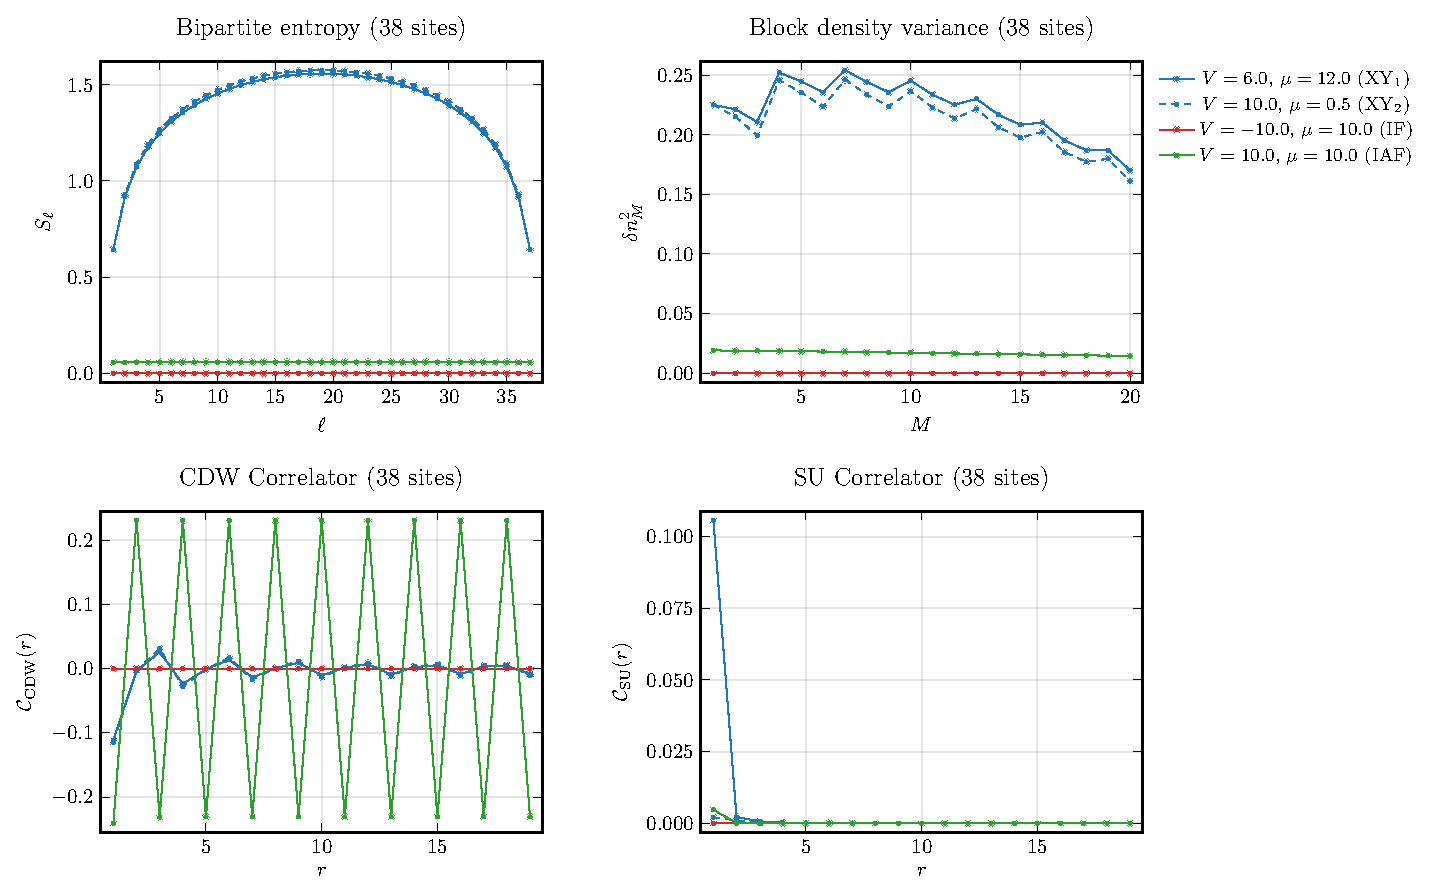
\includegraphics[width=\textwidth]{../Project/analysis/states-properties/compact-plot_L=38.pdf}
	\caption{Compact plot of the four observables listed in Sec.~\ref{subsubsec:single-point-characterization}. Top left: bipartite entropy; top right: block density variance; bottom left: density-density correlator; bottom-right: superconducting correlator. The legend on the top left side listing the four analyzed points refers to all figures.}
	\label{fig:compact-plot}
\end{figure}

Consider Fig.~\ref{fig:compact-plot}: I there sketched the four observables hereby listed computed for $L=14$, for each of the four points analyzed. For each observable, what is shown is the value averaged along the chain; the error is not shown but can be estimated easily by taking the standard deviation across the chain. As a first comment, as expected bipartite entropy and block density variance are indeed significantly larger on the $\mathrm{XY}$ points. Correctly, the $\mathrm{IAF}/\mathrm{MI}_{1/2}$ phase shows both a finite small entropy and a finite small block density variance.

Things get interesting for correlators. Consider the bottom-right plot of Fig.~\ref{fig:compact-plot}, which is, the $\mathrm{CDW}$ density-density correlator plot. The red line represents the density-density correlator for the point $\mathrm{IF}=(-10,10)$ (see Fig.~\ref{fig:points-expected-sfh-phase-diagram.tex}). The state is expected to be unitary filled and Mott insulating, which is, well approximated by
\begin{equation}\label{eq:unitary-state-definition}
	\ket{\Psi} \simeq \ket{\bm{1}} \equiv \bigotimes_{j=1}^L \hat c_j^\dagger \ket{\Omega}
\end{equation}
Correctly the density-density correlation function is identically zero. Recalling the power-law behavior of $\mathcal{C}_\mathrm{CDW}(r)$ of Eq.~\eqref{eq:density-density-correlation-power-law}, such an $r$-dependence signals $K \to 0$. In the same figure, the green line indicates the simulation at the point $\mathrm{IAF}=(10,10)$. Define the states:
\begin{align}
	\ket{\mathrm{e}} &\equiv \bigotimes_{j=1}^{L/2} \hat c_{2j}^\dagger \ket{\Omega}
	&&\text{(even sites filled, odd sites empty)}
	\label{eq:even-state-definition}
	\\
	\ket{\mathrm{o}} &\equiv \bigotimes_{j=1}^{L/2} \hat c_{2j-1}^\dagger \ket{\Omega}
	&&\text{(odd sites filled, even sites filled)}
	\label{eq:odd-state-definition}
\end{align}
For an half-filled Mott-insulating state, the assumption is that the ground-state is dominated by these two,
\[
	\ket{\Psi} \simeq \alpha_\mathrm{e} \ket{\mathrm{e}} + \alpha_\mathrm{o} \ket{\mathrm{o}} + (\cdots)
	\qquad
	\alpha_\mathrm{e}, \alpha_\mathrm{o} \in \mathbb{C}
	\qquad
	\sqrt{\abs{\alpha_\mathrm{e}}^2 + \abs{\alpha_\mathrm{o}}^2} \simeq 1
\]
Moreover, the physical expectation is that $\abs{\alpha_\mathrm{e}} = \abs{\alpha_\mathrm{o}} = 1/2$. For such a situation, is rather easy to show that
\[
	\ev{\delta \hat \rho(i) \delta \hat \rho(j)} = \frac{1}{2} \left[
		\mel{\mathrm{e}}{\hat \rho(i) \hat \rho(j)}{\mathrm{e}} + \mel{\mathrm{o}}{\hat \rho(i) \hat \rho(j)}{\mathrm{o}}
	\right] - \frac{1}{4} = \begin{cases}
		-1/4 &\text{if $\abs{i-j}$ is odd} \\
		1/4 &\text{if $\abs{i-j}$ is even} 
	\end{cases}
\]
an expectation perfectly satisfied by the oscillation visible in Fig.~\ref{fig:compact-plot}, bottom-right panel, green line. Again, recall the expectation of Eq.~\eqref{eq:density-density-correlation-power-law} at half-filling: the correlator oscillation is present, sustained at long distances without suppression -- as before, a signal that $K \to 0$.

\begin{figure}[t]
	\centering
	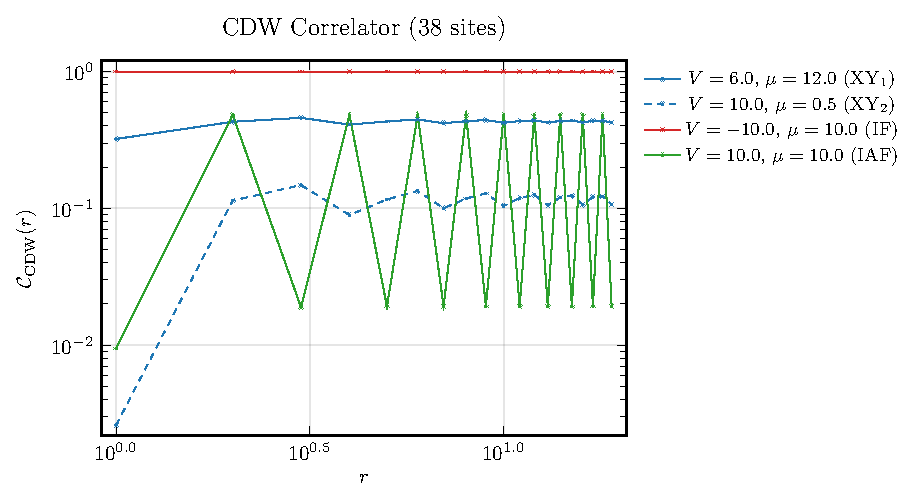
\includegraphics[width=0.6\linewidth]{../Project/analysis/states-properties/cdw-correlator_L=38.pdf}
	\caption{Plot of $\mathcal{C}_\mathrm{CDW}(r)$ limited to the data of the simulation at point $\mathrm{XY}_1 = (6,12)$. Superimposed to the plot, I have plotted a simple Lorentzian decay function with estimated strength $K$. This is not a fit whatsoever.}
	\label{fig:cdw-correlator-zoom-XY1}
\end{figure}

On the same figure, the dashed and solid blue lines (almost indiscernible) represent the correlator computed for the points $\mathrm{XY}_1=(6,12)$ and $\mathrm{XY}_2=(10,0.5)$. Two features are visible: the data oscillate on a length scale bigger than the lattice spacing, and the correlator amplitude is suppressed. I have plotted separately the data for the point $\mathrm{XY}_1 = (6,12)$ in Fig.~\ref{fig:cdw-correlator-zoom-XY1}, superimposing a simple Lorentzian computed via the extracted $K$ parameter for this configuration (reported in Figure),
\[
	- \frac{K}{2\pi^2 r^2}
\]
This is the ``smooth'' part of Eq.~\eqref{eq:density-density-correlation-power-law}. The orange line in Fig.\ref{fig:cdw-correlator-zoom-XY1} is not a fit, is just intended as an illustration. To get more quantitative, one could fit the found data with a three-parameters model from Eq.~\eqref{eq:density-density-correlation-power-law}. Without any good estimation for $\alpha$, I could not do anything more.

\begin{figure}[htbp!]
	\centering
	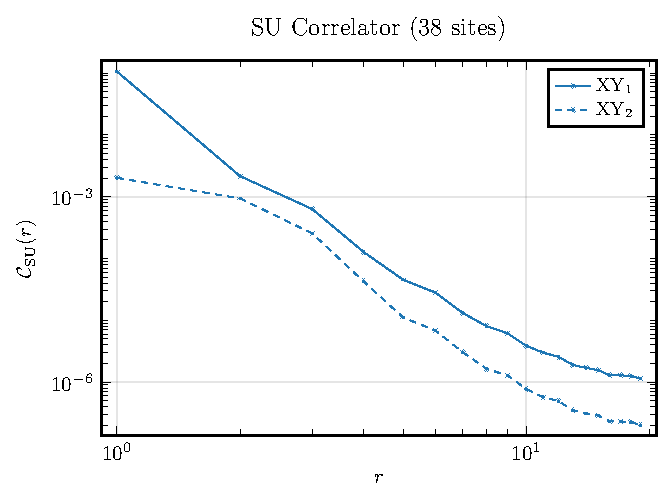
\includegraphics[width=0.6\linewidth]{../Project/analysis/states-properties/su-correlator_L=38.pdf}
	\caption{Logarithmic plot of $\mathcal{C}_\mathrm{SU}(r)$. The power-law decay is qualitatively visible and would require deeper and quantitative investigation.}
	\label{fig:su-correlator-loglog}
\end{figure}

Finally, on the bottom right panel of Fig.~\ref{fig:compact-plot} I have reported the simulated data for $\mathcal{C}_\mathrm{SU}(r)$. For what is intelligible in the plot, coherently with expectations, the Mott-insulating states' correlators vanish identically. For the sake of intelligibility, I also plotted the $\mathrm{XY}$ data on a \texttt{:loglog} scale in Fig.~\ref{fig:su-correlator-loglog}. For both the points simulated, the decay is vaguely power-law with some evident deviations at big distance. I reconnect this last effect to the finite size: the finite nature of the chain introduces another length scale over which correlations decay, related directly to $L$. Over this length scale decay is expected to be exponential-like. Regarding Fig.~\ref{fig:su-correlator-loglog}, there is nothing much I can say apart from \textit{much} qualitative comments. I tried comparing with a power-law decay using the estimated $K$, as in Fig.~\ref{fig:cdw-correlator-zoom-XY1}, but results were unsatisfying. Evidently the simulations are not good enough to represent these correlations.

\subsubsection{Observables heatmaps}

\begin{figure}
	\centering
	\subfloat[][Density heatmap.]{
		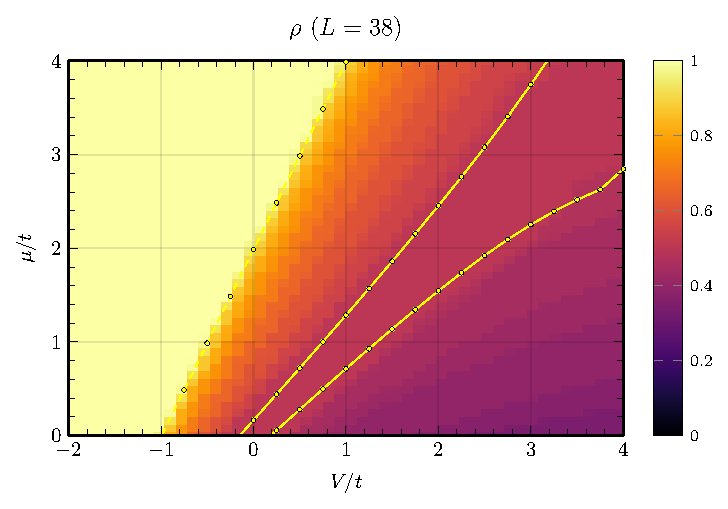
\includegraphics[height=0.35\textwidth]{
			../Project/analysis/heatmap/density_L=38.pdf
		}\label{subfig:density-heatmap}
	}
	\subfloat[][Block density variance heatmap.]{
		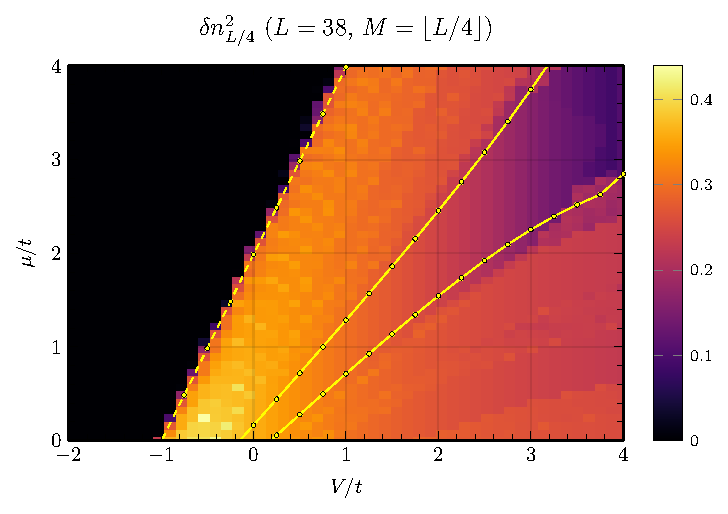
\includegraphics[height=0.35\textwidth]{
			../Project/analysis/heatmap/block-density-variance_L=38.pdf
		}\label{subfig:block-density-variance-heatmap}
	}
	\caption{The averaged density heatmap for the DMRG solved ground state of the spinless Fermi-Hubbard model is shown in Fig~\ref{subfig:density-heatmap}. Superimposed and with the same criteria as in Fig.~\ref{fig:phase-boundaries} are the expected phase boundaries. Fig.~\ref{subfig:block-density-variance-heatmap} depicts the average density variance across a block of sites of length $M = \lfloor L/4 \rfloor$.}
	\label{fig:density-heatmaps}
\end{figure}

In this last section I sketch some relevant observables heatmaps. Results are described qualitatively but give space to deep understanding of how the (finite-size) phases are made.

\paragraph{Density.} I start by commenting the results shown in Fig.~\ref{fig:density-heatmaps}. The first and simplest observable is the average particle density along the chain, shown as a heatmap in Fig.~\ref{subfig:density-heatmap}. As expected the left-side $\mathrm{IF}/\mathrm{MI}_1$ phase is unitary filled, while the expected $\mathrm{IAF}/\mathrm{MI}_{1/2}$ is almost uniformly half-filled. Due to finite size, which implies finite particle number, in the expected $\mathrm{XY}$ phase uniform-density domains borders are clearly visible. These correspond to single particles removal.

Interestingly, at zero chemical potential (no system-environment matter exchange) the expected density at strong NN repulsion is less than half. To alternate particles and holes in not enough to gain energy: residual subdominant hopping makes the ground state converge onto a less populated state.

\paragraph{Block density variance.} Fig.~\ref{subfig:block-density-variance-heatmap} shows the block density variance $\ev{ \delta \hat n_{M}^2 }$ as a heatmap for $M = \lfloor L/4 \rfloor$. For the $\mathrm{IF}/\mathrm{MI}_1$ phase, the variance of density along the block is null -- a consequence of the robust ground-state $\ket{\Psi} \simeq \ket{\bm{1}}$ as defined in Eq.~\eqref{eq:unitary-state-definition}.
Similarly, the dominant contribution to the $\mathrm{IAF}/\mathrm{MI}_{1/2}$ phase is given by the states $\ket{\mathrm{e}}$ and $\ket{\mathrm{o}}$ as defined respectively in Eqns.~\eqref{eq:even-state-definition}, \eqref{eq:odd-state-definition}. Separately, each of these states is a number operator eigenstate and thus has zero density variance on each site and on every block. For a state in $\mathrm{Span}\lbrace \ket{\mathrm{e}}, \ket{\mathrm{o}} \rbrace$ the variance over a block is expected to be small:
\[
	\ket{\Psi} = \frac{1}{\sqrt{1 + \abs{\gamma}^2}} \ket{\mathrm{e}} + \frac{\gamma}{\sqrt{1 + \abs{\gamma}^2}} \ket{\mathrm{o}}
	\qquad
	\gamma \in \mathbb{C}
\]
and
\[
	\mel{\Psi}{\hat n_j}{\Psi} = \frac{1+(-1)^j}{2} \frac{1}{1 + \abs{\gamma}^2} + \frac{1-(-1)^j}{2} \frac{\abs{\gamma}^2}{1 + \abs{\gamma}^2} = 		\mel{\Psi}{\hat n_j^2 }{\Psi}
\]
Since
\[
	\left(
		\frac{1\pm(-1)^j}{2}
	\right)^2 = \frac{1\pm(-1)^j}{2}
	\qquad\text{and}\qquad
	\frac{1\pm(-1)^j}{2} \frac{1\mp(-1)^j}{2} = 0
\]
this implies using some basic algebra
\[
	\mel{\Psi}{\hat n_j^2 }{\Psi} - \mel{\Psi}{\hat n_j}{\Psi}^2 = \frac{\abs{\gamma}^2}{\left(1 + \abs{\gamma}^2\right)^2}  \le \frac{1}{4}
\]
the last inequality being trivial to prove and satisfied $\forall \gamma \in \mathbb{C}$. One can show easily that if the state is not dominated by $\ket{\mathrm{e}}, \ket{\mathrm{o}}$ and the number of particles on the chain is allowed to fluctuate -- as is in the superpositions composing the $\mathrm{XY}$ ground states -- the $j$-site variance increases. Such difference becomes even sharper when considering a block of sites of length $M$ instead of a single site $j$\footnote{
	I will not show this here, being the proof purely algebraic and not so interesting. This behavior essentially arises because of the appearance of connected density-density correlation functions, whose power-law decay in $\mathrm{XY}$ phase produces the ``boost'' of the observable.
}. In Fig.~\ref{subfig:block-density-variance-heatmap} such a behavior is observed, becoming more and more important as we approach the top-right side of the picture, coherently with the theoretical expectations of Fig.~\ref{fig:expected-sfh-phase-diagram}. This last property is interesting, because it signals that the finite-size version of the gapped $\mathrm{IAF}/\mathrm{MI}_{1/2}$ phase extends over a broad region but remains most similar to its thermodynamic limit in the correct part of the phase diagram.
	
\begin{figure}
	\centering	
	\subfloat[][Overlap with $\ket{\bm{1}}$.]{
		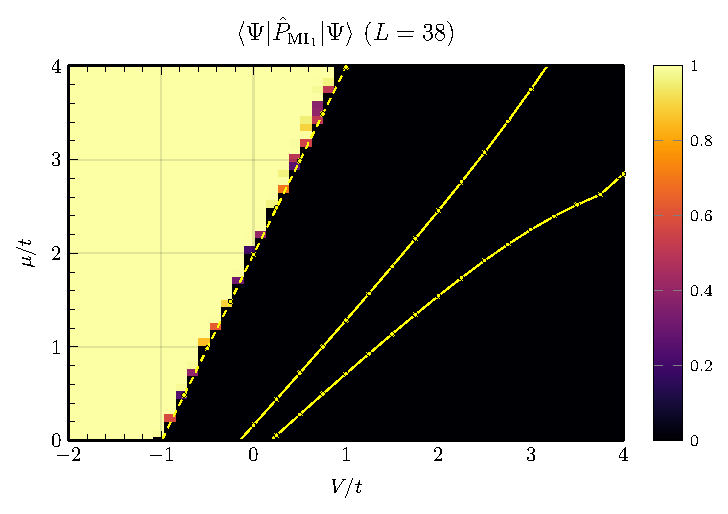
\includegraphics[height=0.35\textwidth]{
			../Project/analysis/heatmap/uMI_projection_L=38.pdf
		}\label{subfig:uMI-projection-heatmap}
	}
	\subfloat[][Overlap with $\mathrm{Span}\lbrace \ket{\mathrm{e}}, \ket{\mathrm{o}} \rbrace$.]{
		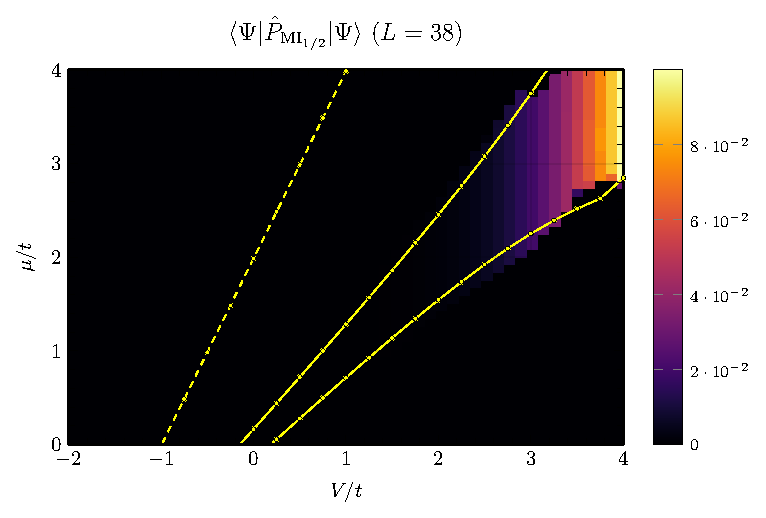
\includegraphics[height=0.35\textwidth]{
			../Project/analysis/heatmap/hMI_projection_L=38.pdf
		}\label{subfig:hMI-projection-heatmap}
	}\caption{In Fig.~\ref{subfig:uMI-projection-heatmap} the projection of the ground-state onto the pure $\mathrm{IF}/\mathrm{MI}_1$ subspace is shown; such subspace is spanned by $\ket{\bm{1}} \equiv \ket{11\cdots1}$. Similarly, Fig.~\ref{subfig:hMI-projection-heatmap} shows the projection of the ground-state onto the pure $\mathrm{IAF}/\mathrm{MI}_{1/2}$ subspace, given by $\mathrm{Span}\lbrace \ket{\mathrm{e}}, \ket{\mathrm{o}} \rbrace$.}
\end{figure}

\paragraph{Projection onto Mott subspaces.} A good confirmation of the assumptions of the above paragraph is to check directly how much the ground-state is projected onto a given Mott subspace. Let me start by the $\mathrm{IF}/\mathrm{MI}_1$ phase. Let me define
\[
	\hat{\mathrm{P}}_{\mathrm{MI}_1} = \op{\bm{1}}{\bm{1}}
\]
Evidently, if
\[
	\ket{\Psi} = \alpha_{\bm{1}} \ket{\bm{1}} + \sum_\psi \alpha_\psi \ket{\psi}
\]
being $\ket{\psi}$ any other state and the $\alpha$s the amplitudes, we get
\[
	\ev{\hat{\mathrm{P}}_{\mathrm{MI}_1}} = \abs{\alpha_{\bm{1}}}^2
\]
which is the probability for the state to coincide (up to an irrelevant phase) with $\ket{\bm{1}}$. Consider Fig.~\ref{subfig:uMI-projection-heatmap}: inside the expected $\mathrm{IF}/\mathrm{MI}_1$ region, the convergence of the simulated state on $\ket{\bm{1}}$ is absolute. Outside, the simulated state is (obviously) orthogonal to $\ket{\bm{1}}$. I defined this MPO simply as
\begin{lstlisting}[language=julia]
function GetUnitaryMIProjector(
		sites::Any
	)::MPO

	L = length(sites)
	
	states = ["1" for j in 1:L]		# 1111...
	u = MPS(sites, states)			# Unitary-filled state
	
	UP = projector(u)
	return UP

end
\end{lstlisting}

Similarly, let me define 
\[
	\hat{\mathrm{P}}_{\mathrm{MI}_{1/2}} = \op{\mathrm{e}}{\mathrm{e}} + \op{\mathrm{o}}{\mathrm{o}}
\]
the projector onto the $\mathrm{IAF}/\mathrm{MI}_{1/2}$ phase. With analogous notation as above,
\[
	\ev{\hat{\mathrm{P}}_{\mathrm{MI}_{1/2}}} = \abs{\alpha_\mathrm{e}}^2  + \abs{\alpha_\mathrm{o}}^2
\]
which is the probability for the ground-state of being in the $\mathrm{Span}\lbrace \ket{\mathrm{e}}, \ket{\mathrm{o}} \rbrace$ subspace. The MPO was initialized as:
\begin{lstlisting}[language=julia]
function GetHalfMIProjector(
		sites::Any
	)::MPO
	
	L = length(sites)
	
	states = [isodd(j) ? "0" : "1" for j in 1:L] # 0101...
	e = MPS(sites, states)						 # Even-filled state
	
	states = [isodd(j) ? "1" : "0" for j in 1:L] # 1010...
	o = MPS(sites, states)						 # Odd-filled state
	
	E = projector(e) # Normalized projector
	O = projector(o) # Normalized projector
	HP = E+O
	return HP

end
\end{lstlisting}
Now, I expected the projection probability to saturate quickly to unity with better and better approximation as the chain got larger. Instead, as is visible in Fig.~\ref{subfig:hMI-projection-heatmap}, it turns out that the simulated state lies in the $\mathrm{Span}\lbrace \ket{\mathrm{e}}, \ket{\mathrm{o}} \rbrace$ subspace with a probability of approximately $10\%$. Correctly, the projection probability seems to increase by moving to the top-right corner. Of course I expected way better results. I tried changing the DMRG parameters (specifically \texttt{nSweeps}) but noticed no measurable improvement: the algorithm converges quickly. I tried simulating different $(V/t,\mu/t)$ choices at increasing lattice dimension. 

\begin{table}
	\centering
	\begin{tabular}{r c c c c c}
		\multicolumn{6}{c}{$\langle \hat{\mathrm{P}}_{\mathrm{MI}_{1/2}} \rangle \Big|_{L,V/t,\mu/t}$} \\
		\toprule
		& \multicolumn{5}{c}{$V/t=\mu/t$}\\
		\cmidrule{3-6}
		$L$ && $5$ & $10$ & $20$ & $50$ \\
		\midrule
		$ 38 $ && $ 0.238 $ & $ 0.692 $ & $ 0.912 $ & $ 0.985 $ \\
		$ 54 $ && $ 0.127 $ & $ 0.591 $ & $ 0.876 $ & $ 0.979 $ \\
		$ 70 $ && $ 0.068 $ & $ 0.504 $ & $ 0.842 $ & $ 0.973 $ \\
		$ 86 $ && $ 0.036 $ & $ 0.43 $ & $ 0.809 $ & $ 0.967 $ \\
		$ 102 $ && $ 0.019 $ & $ 0.366 $ & $ 0.777 $ & $ 0.96 $ \\
		$ 118 $ && $ 0.01 $ & $ 0.312 $ & $ 0.747 $ & $ 0.954 $ \\
		$ 134 $ && $ 0.006 $ & $ 0.266 $ & $ 0.717 $ & $ 0.948 $ \\
		$ 150 $ && $ 0.003 $ & $ 0.227 $ & $ 0.689 $ & $ 0.942 $ \\
		\bottomrule
	\end{tabular}
	\caption{Probability for the simulated ground state of the model with $V/t = \mu/t$ as specified in the first row to be in the subspace $\mathrm{Span}\lbrace \ket{\mathrm{e}}, \ket{\mathrm{o}} \rbrace$ at increasing chain lengths $L$.}
	\label{tab:MI1/2-projections}
\end{table}

Consider Tab.~\ref{tab:MI1/2-projections}: there are reported the results of the expectation value of the projector over ground states simulated at increasing ratios $V/t = \mu/t$ -- which is, on the top-right diagonal. The last column (calculated in the extreme anti-ferromagnetic parametrization), correctly, saturates at almost unity. Lowering the parameters and increasing the lattice length, interestingly the probability decreases down to extremely small values (below $1\%$ for $L>118$, $V/t=\mu/t=5$). I have tried using more generous DMRG parameters, but results did not improve much. Probably, these data are explained by the fact that -- even if algebraically simple -- the $\mathrm{IAF}$ ground state is non-locally entangled. This means, even if the number of many-body states entangled is low, in the physical ground state in thermodynamic limit each site is entangled with every other -- a condition of low long-range entanglement Finite-Size DMRG struggles to reproduce over finite lengths. Probably the simulated states is more similar to a collection of cluster of sites entangled Anti-Ferromagnetically.

A possible measurement one could carry out (I did not) is the averaged projection onto finite-size Anti-Ferromagnetic local projectors,
\[
	\hat{\mathrm{P}}_{\mathrm{MI}_{1/2}}^M =
	\frac{1}{L} \sum_{s=1}^{L}
		\left[
			\bigotimes_{j=s}^{s+M} \hat c_{2j}^\dagger \op{\Omega}{\Omega} \bigotimes_{k=s}^{s+M} \hat c_{2k}
			+
			\bigotimes_{j=s}^{s+M} \hat c_{2j-1}^\dagger \op{\Omega}{\Omega} \bigotimes_{k=s}^{s+M} \hat c_{2k-1}
		\right]
\]
which is, the equivalent of the projector analyzed above but limited to blocks of length $M$ and averaged over different blocks.

\paragraph{Luttinger parameters.} 

\begin{figure}
	\centering	
	\subfloat[][Charge compressibility.]{
		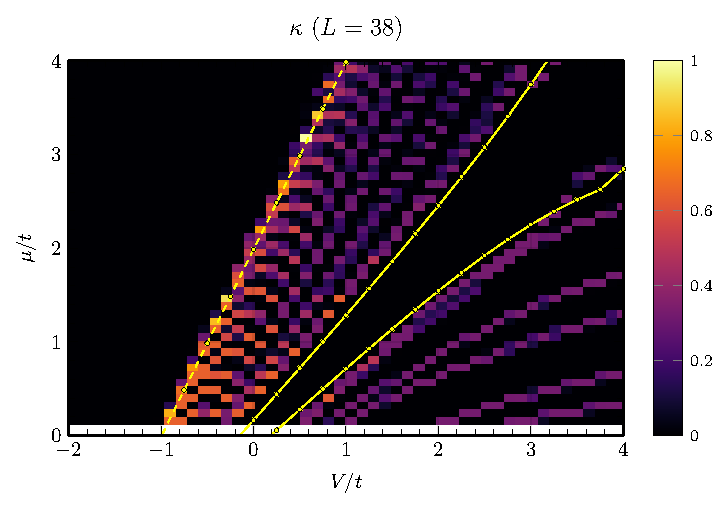
\includegraphics[height=0.35\textwidth]{
			../Project/analysis/heatmap/compressibility_L=38.pdf
		}\label{subfig:compressibility-heatmap}
	}
	\subfloat[][Charge stiffness.]{
		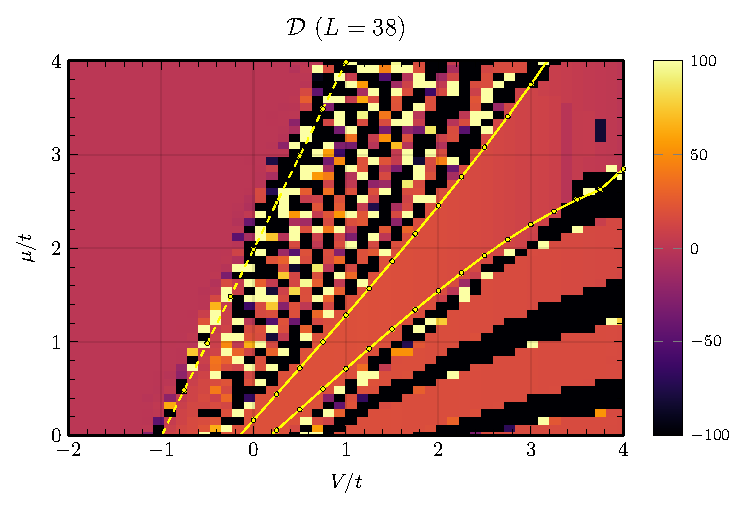
\includegraphics[height=0.35\textwidth]{
			../Project/analysis/heatmap/stiffness_L=38.pdf
		}\label{subfig:stiffness-heatmap}
	}
	\caption{In Fig.~\ref{subfig:compressibility-heatmap}, the ground state compressibility is reported. The low part of the plot (small chemical potential) has been omitted: compressibility was here computed by the means of finite differences, a technique requiring cached data from previous simulations. Finite differentiation is also responsible for the smearing of the heatmap across the phase boundaries. In Fig~\ref{subfig:stiffness-heatmap} the charge stiffness for a small flux threading the chain is plotted.}
\end{figure}

Finally, I explored roughly the behavior of charge compressibility $\kappa$ and charge stiffness $\mathcal{D}$, as explained in Sec.~\ref{subsec:what-i-would-have-liked-to-do-(better)}. Both observables are extracted by the means of finite derivatives: $\kappa$, by looking at the density difference at two close chemical potentials; $\mathcal{D}$, by looking at the current response to small fluxes, which is, the energy derivative response.

Fig.~\ref{subfig:compressibility-heatmap} shows a heatmap of the finite-size compressibility. Taking into account the roughness of the simulation, coherence with the expectations is acceptable. The two interesting Mott-insulating regions are almost uniformly non compressible, a signature of the presence of a gap. Outside, fluctuations in compressibility are visible. It must be noted that, for an infinitely long chain (the continuum limit) the step-like regions of gradually decreasing density of Fig.~\ref{subfig:density-heatmap} between the two Mott phases degenerate into a continuum. In other words: moving from the unitary-filled to the half-filled region, the density varies continuously. For a small finite chain, the finite-size effect is the step-like variation of density, a feature giving rise to the aforementioned fringes as well as the zero-compressibility regions in the bottom right corner of the phase diagram \ref{subfig:compressibility-heatmap}. These regions are not generated by a thermodynamically gapped phase, rater by the finite-size nature of the simulation.

In Fig.~\ref{subfig:stiffness-heatmap} the charge stiffness heatmap is reported. Similar observations as for the charge compressibility hold for $\mathcal{D}$. The $\mathrm{IF}/\mathrm{MI}_1$ phase is stiff: given some flux threading the chain, static Mott-localization gives null current response. A non-zero current response requires the possibility of hopping, which in turn requires a filled site near an empty site. No infinitesimal flux can be responsible of the global synchronized rotation of all the fermions in the unitary-filled state.
The $\mathrm{IAF}/\mathrm{MI}_{1/2}$ presents a small finite positive stiffness, gradually decreasing to zero in the top-right corner of Fig.~\ref{subfig:stiffness-heatmap}. Analogous considerations as for the unitary filled state hold here, and Mott localization explains the stiffness. Outside, as for $\kappa$, fringes are visible. Interestingly, changes in parity appear to cause current response to diverge negatively.

Recall now Eqns.~\eqref{eq:u-K-formulas},
\[
	u = \sqrt{\frac{\mathcal{D}}{\pi\kappa}}
	\qquad\text{and}\qquad
	K = \sqrt{\pi\kappa\mathcal{D}}
\]
Compressibility and charge stiffness, multiplied and divided, are connected to the Luttinger parameters $u$ and $K$. The two parameters completely govern the bosonization description of a one-dimensional spinless fermionic system. Most importantly, as explained in Sec.~\ref{subsubsec:meaning-of-the-luttinger-parameter-K}, if $K < 1$ the equivalent interaction between bosons is repulsive and gives rise to a $\mathrm{CDW}$ behavior. If $K > 1$, the interaction is attractive and the main dynamics is superfluid.

\begin{figure}
	\centering	
	\subfloat[][$u$ Luttinger paramter.]{
		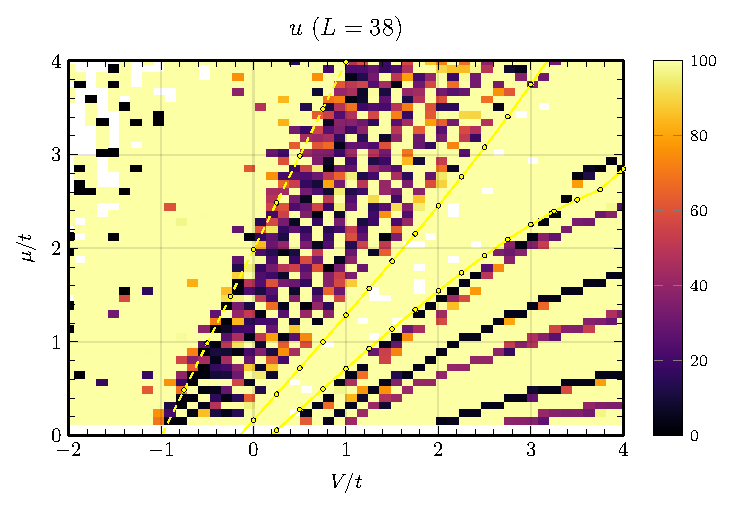
\includegraphics[height=0.35\textwidth]{
			../Project/analysis/heatmap/u-Luttinger_L=38.pdf
		}\label{subfig:u-Luttinger-heatmap}
	}
	\subfloat[][$K$ Luttinger parameter.]{
		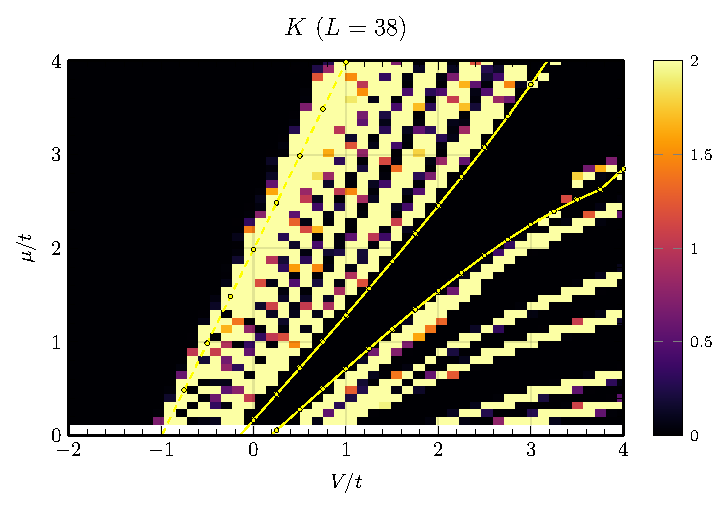
\includegraphics[height=0.35\textwidth]{
			../Project/analysis/heatmap/K-Luttinger_L=38.pdf
		}\label{subfig:K-Luttinger-heatmap}
	}
	\caption{Honestly, I have no idea what is going on in Fig.~\ref{subfig:u-Luttinger-heatmap}, showing the renormalized velocity $u$. In order to make the data intelligible I had to apply a cutoff of $100$. In Fig.~\ref{subfig:K-Luttinger-heatmap} the heatmap for the Luttinger parameter $K$ is sketched. The low part has been cut off because of the finite-differences method used to compute $\kappa$.}
	\label{fig:Luttinger-heatmaps}
\end{figure}

Comically, the $u$ and $K$ heatmaps of Fig.~\ref{fig:Luttinger-heatmaps} -- which should have been the entire point of this whole project -- are not so satisfying. On one hand, the plot for $u$ in Fig.~\ref{subfig:u-Luttinger-heatmap} -- apart from the general structure -- is not insightful, oscillates strangely in the robust ferromagnetic phase and is evidently suffering from some numerical error in calculating $u$ starting from $\kappa$, $\mathcal{D}$. On the other hand Fig.~\ref{subfig:K-Luttinger-heatmap} shows -- as expected -- a strongly suppressed $K$ in the Mott-insulating region (signaling a $\mathrm{CDW}$ kind of order), while outside the same parameter oscillates and reaches values much bigger than $1$. Note that the heatmap has been limited to the values $[0,2]$ for intelligibility reasons. Apart from this consideration, which confirms expectations, not much more can be said.

Let me close with a positive note. At least, the heatmap for the Luttinger parameter $K$ in Fig.~\ref{subfig:K-Luttinger-heatmap} makes sense in the bosonization framework. Remembering the many turns of this project, I could not have asked for more.
